\documentclass[runningheads]{llncs}
\usepackage{amsmath,amssymb}
\usepackage{graphicx,rotating}
\usepackage[font=small]{subfig,caption}
\usepackage{algorithm2e}
\usepackage{todonotes,lineno,paralist,soul}
\usepackage{placeins,rotating,hyperref}
\graphicspath{{figures/}}

\author{Michael~A.~Bekos, Henry~F\"orster, Christian~Geckeler, Lukas Holl\"ander, Michael~Kaufmann, Amad\"aus~Spallek, Jan~Splett}
\authorrunning{M.~A.~Bekos et al.}
\title{A Heuristic Approach towards Drawings of Graphs with High Crossing Resolution}
\titlerunning{Drawings of Graphs with High Crossing Resolution}

\institute{
Wilhelm-Schickhard-Institut f\"ur Informatik, Universit\"at T\"ubingen, Germany\\
\texttt{\{bekos,foersth,mk\}@informatik.uni-tuebingen.de}\\
\texttt{\{christian-marius.geckeler,jan-lukas.hollaender,amadaeus.spallek,jan.splett\} @student.uni-tuebingen.de}
}

% ============================================================
\begin{document}
\maketitle
\linenumbers
% ==================================================================

\begin{abstract}
The \emph{crossing resolution} of a non-planar drawing of a graph is the minimum angle formed by any pair of crossing edges. Recent experiments have shown that the larger the crossing resolution is, the easier it is to read and interpret a drawing of a graph. However, maximizing the crossing resolution turns out to be an NP-hard problem in general and only heuristic algorithms are known that are mainly based on appropriately adjusting force-directed algorithms. 
 
In this paper, we propose a new randomization-based heuristic algorithm for the crossing resolution maximization problem and we experimentally compare it against the known ones from the literature. Our experimental evaluation indicates that the new heuristic produces drawings with significantly better crossing resolution, but this comes at the cost of slightly higher running time, especially when the input graph is large and dense. 
\end{abstract}

\section{Introduction}
\label{sec:introduction}

In Graph Drawing, there exists a really rich literature and a wide range of techniques for drawing planar graphs; see, e.g.,~\cite{DBLP:journals/combinatorica/FraysseixPP90,DBLP:conf/gd/GutwengerM98,DBLP:journals/algorithmica/Kant96}. However, drawing a non-planar graph, and in particular when it does not have some special structure (e.g., degree restricted), is a difficult and challenging task, mainly due to the edge crossings which negatively affect the drawing's quality~\cite{DBLP:journals/iwc/Purchase00}. As a result, the enstablished techniques are significantly fewer (e.g., crossing minimization heuristics~\cite{DBLP:journals/algorithmica/EadesW94,DBLP:journals/tsmc/SugiyamaTT81}, energy-based layout algorithms~\cite{DBLP:journals/congnum/Eades84,DBLP:journals/spe/FruchtermanR91}); for an overview refer to~\cite{DBLP:books/ph/BattistaETT99,DBLP:conf/dagstuhl/1999dg,DBLP:reference/crc/2013gd}.

In this context, Huang et al.~\cite{DBLP:conf/apvis/Huang07,DBLP:journals/vlc/HuangEH14} a decade ago introduced some important experimental evidence (through a series of eye-tracking experiments), that edge crossings may not negatively affect the drawing's quality too much (and therefore the human's ability to read and interpret it), when the angles formed by the crossing edges are large. In other words, while prior to these experiments it was commonly accepted that mainly the number of crossings is the most important parameter for judging the quality and readability of a non-planar graph drawing, it turned out that the types of edge crossings also matter. As a result, a new and prominent research direction was initiated, which is recognized under the term ``beyond planarity''~\cite{Shonan2016,Dagstuhl2016,SoCG2017} and mainly focuses on graphs and their properties, when different constraints on the types of edges crossings are imposed; refer to~\cite{DBLP:journals/corr/abs-1804-07257} for a recent survey. 

Formally, the minimum angle formed by any pair of crossing edges in a drawing is refered to as its \emph{crossing resolution}. Analogously, the crossing resolution of a graph is defined as the maximum crossing resolution over all its drawings. Clearly, the crossing resolution of a non-planar graph is at most $90^\circ$, while a graph that admits a drawing with crossing resolution $90^\circ$ is called \emph{right-angle-crossing} graph or \emph{RAC} graph, for short; refer to Figure~\ref{fig:examples} for an illustration. For these graphs, several results, mostly of theoretical nature, are known (refer to Section~\ref{sec:relatedwork} for a short overview). Notably, RAC graph are sparse (they contain at most $4n-10$ edges~\cite{DBLP:journals/tcs/DidimoEL11}, where $n$ denotes the number of  vertices), while deciding whether a graph is RAC is NP-hard~\cite{DBLP:journals/jgaa/ArgyriouBS12}.

\begin{figure}[t!]
	\centering
	\subfloat[\label{fig:k5} {}]{
	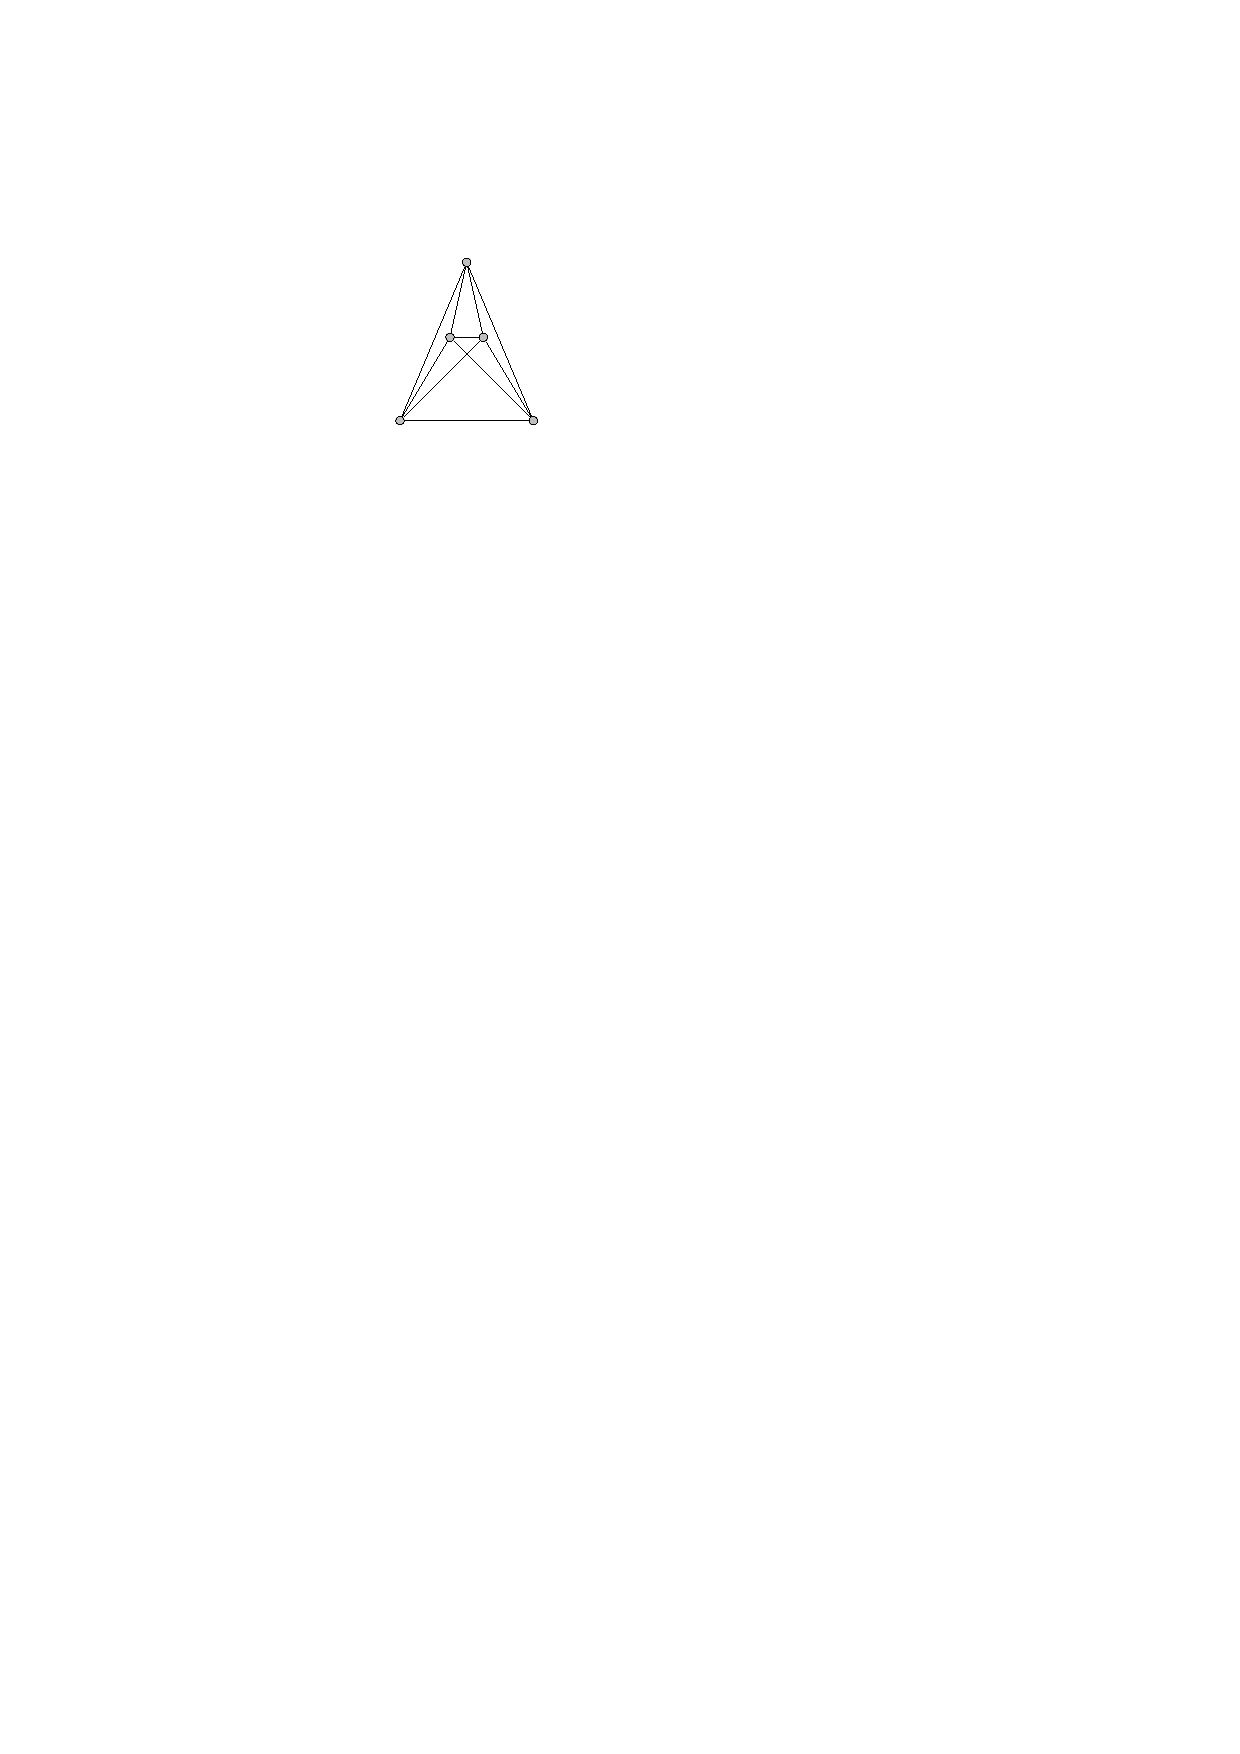
\includegraphics[page=1]{figures/examples}}
	\hfil
	\subfloat[\label{fig:k6} {}]{
	\includegraphics[page=2]{figures/examples}}
	\caption{%
	(a)~A RAC drawing of the complete graph $K_5$, and
	(b)~a drawing of the complete graph $K_6$, whose crossing resolution is arbitrarily close to $90^\circ$.}
	\label{fig:examples}
\end{figure} 

The latter result is already an indication that the problem of finding drawings with high crossing resolution might also be difficult, even though, formally, its complexity has not been settled yet for values of the crossing resolution smaller than $90^\circ$. Also, the literature is significantly more limited, when restricting the crossing resolution to be smaller than $90^\circ$, as also evidenced by Section~\ref{sec:relatedwork}. 

From a practical point of view, we are only aware of two methods that aim at drawings with high crossing resolution; both of them are adjustments of force-directed algorithms~\cite{DBLP:journals/congnum/Eades84}. The first one is due to Huang, Eades, Hong and Lin~\cite{DBLP:journals/vlc/HuangEHL13}, while the second one is due to Argyriou, Bekos and Symvonis~\cite{DBLP:journals/cj/ArgyriouBS13}. Common in both algorithms is that they apply appropriate forces on the endvertices of every pair of crossing edges. Each of the two algorithms uses a different way to compute (the direction and the magnitude of) the forces, but the underlying idea in both algorithms is the same: the smaller the corresponding crossing angles are, the larger are the magnitudes of the forces applied at their endvertices. 

In this paper, we approach the crossing resolution maximization problem from a different perspective. We suggest a simple and quite intuitive randomization method for computing drawings with high crossing resolution, which, in a sense, mimics the way a human would try to increase the crossing resolution of a drawing. How would one try to increase the crossing resolution of a given drawing? First, she would try to identify the pair of edges that define the crossing resolution of the drawing (we call them \emph{critical} edges); then, she would try to move an endvertex of this pair (which we choose at random), hoping that by this move the crossing resolution will increase. Of course, we cannot consider all possible positions for the vertex to be moved. Instead, we consider a small set of randomly generated ones. Then, if there exists a position among them, that does not lead to a reduction of the crossing resolution, we simply move the vertex to this~position.

In general, randomization is a technique that has not been deeply examined in Graph Drawing, as it seems to be difficult to compute the expected quality of the produced drawings; a notable exception is the randomized approach by Goldschmidt and Takvorian~\cite{DBLP:journals/networks/GoldschmidtT94} for computing large planar subgraphs. Since we could not provide any theoretical guarantee on the expected quality of the produced drawings as well (mainly due to the nature of the problem itself), we decided to follow a more practical approach. To this end, we implemented our algorithm and the ones presented in~\cite{DBLP:journals/vlc/HuangEHL13} and~\cite{DBLP:journals/cj/ArgyriouBS13}, and we experimentally compared the crossing resolutions of the drawings produced by them for standard benchmark graphs (such as the Rome and the North graphs) that are widely used in Graph Drawing for comparing different drawing algorithms. Our experimental evaluation indicates that our new method significantly outperforms the ones that are based on adjustments of force-directed algorithms~\cite{DBLP:journals/vlc/HuangEHL13,DBLP:journals/cj/ArgyriouBS13} in terms of crossing resolution, but this comes at the cost of slightly worse running time, especially for large and dense graphs. 

\paragraph{Preliminaries:}
Unless otherwise specified, in this paper we consider simple undirected graphs. Let $G=(V,E)$ be such a graph. The degree of vertex $u\in V$ of $G$ is denoted by $d(u)$. The degree $d(G)$ of  graph $G$ is defined as the maximum degree of its vertices, i.e., $d(G)=\max_{u\in V}d(u)$.
%
Given a drawing $\Gamma(G)$ of $G$, we denote by $p(u)=(x_u,y_u)$ the position of vertex $u \in V$ of $G$ in $\Gamma(G)$. %For a pair of vertices $u,v\in V$ of $G$, the unit-length vector from $p(u)$ to $p(v)$ is denoted as $\overrightarrow{p(u)p(v)}$, while the line segment delimited by $p(u)$ and $p(v)$ as $\overline{p(u)p(v)}$.

\paragraph{Structure of the paper:}
The remainder of this paper is structured as follows. Section~\ref{sec:relatedwork} overviews related works. 
%In Section~\ref{sec:preliminaries}, we introduce preliminary notions and the notation used throughout the paper. 
Our algorithm is presented in detail in Section~\ref{sec:algorithm} and is experimentally evaluated against the ones of Huang et al.~\cite{DBLP:journals/vlc/HuangEHL13} and Argyriou et al.~\cite{DBLP:journals/cj/ArgyriouBS13} in Section~\ref{sec:experiments}. We conclude in Section~\ref{sec:conclusions} with interesting open problems and future~directions.
 
\section{Related Work}
\label{sec:relatedwork}

As already mentioned, the study of the crossing resolution maximization problem has mainly focused on (properties of) RAC graphs, that is, on the optimal case of the crossing resolution maximization problem. The study was initiated by Didimo et al.~\cite{DBLP:journals/tcs/DidimoEL11}, who showed that an $n$-vertex RAC graph has at most $4n-10$ edges. 
Angelini et al.~\cite{DBLP:journals/jgaa/AngeliniCDFBKS11} presented results for two interesting variants, in which the input graph is either an acyclic digraph or a graph of bounded vertex degree. Argyriou et al.~\cite{DBLP:journals/jgaa/ArgyriouBS12} showed that the problem of deciding whether a graph is RAC is NP-hard. Didimo et al.~\cite{DBLP:journals/ipl/DidimoEL10} completely characterized the complete bipartite RAC graphs. Di~Giacomo et al.~\cite{DBLP:journals/algorithmica/GiacomoDEL14}, and Hong and Nagamochi~\cite{DBLP:conf/wg/HongN15} studied variants, in which the vertices of the input graph are restricted on two parallel lines and on the circumference of a circle, respectively. Eades and Liotta~\cite{DBLP:journals/dam/EadesL13} showed that the optimal RAC graphs (i.e., those of maximum density) are 1-planar (i.e., they admit drawings in which each edge is crossed at most once). Deciding, however, whether a 1-planar graph is RAC is NP-hard~\cite{DBLP:journals/tcs/BekosDLMM17}. Other relationships between the class of RAC graphs and subclasses of 1-planar graphs have also been studied by Bachmaier et al.~\cite{DBLP:journals/dam/BachmaierBHNR17} and Brandenburg et al.~\cite{DBLP:journals/tcs/BrandenburgDEKL16}. Note that the problem of finding RAC drawings has been also studied in the presence of bends; see e.g.~\cite{DBLP:journals/jgaa/AngeliniCDFBKS11,DBLP:journals/comgeo/ArikushiFKMT12,DBLP:journals/tcs/DidimoEL11,DBLP:journals/mst/GiacomoDLM11}. 

To the best of our knowledge, there is only one work, by Dujmovic et al.~\cite{DBLP:journals/cjtcs/DujmovicGMW11}, which studies the crossing resolution maximization problem by relaxing the right-angle constraint on the crossing angles of the computed drawings. More precisely, in their work, Dujmovic et al.~\cite{DBLP:journals/cjtcs/DujmovicGMW11} proved that an $n$-vertex graph, whose crossing resolution is at least $\alpha$ (in radians) has at most $(3n-6)\pi/\alpha$ edges. Corresponding density results for the case, in which few bends are allowed along each edge, are known by Ackerman et al.~\cite{DBLP:journals/siamdm/AckermanFT12} and Di Giacomo et al.~\cite{DBLP:journals/mst/GiacomoDLM11}.  

An immediate observation emerging from the above literature overview is that the focus of the study of the crossing resolution maximization problem has been primarily on theoretical aspects of the problem. Most of the approaches that could be useful in practise are based on adjustments of force-directed techniques~\cite{DBLP:journals/congnum/Eades84}, according to which a graph is modelled as a physical system with forces acting on it, and a (good) drawing is obtained by an equilibrium of the system; for an introduction and a discussion of several variants refer to~\cite{DBLP:books/ph/BattistaETT99}. %Actually, the absence of approaches for computing drawings with high crossing resolution in practice is rather obvious and it can be justified, up to a certain point, by the fact that the problem turns to be NP-hard, when asking for drawings with optimal crossing resolution. 

More concretely, from an applicative point of view, Didimo et al.~\cite{DBLP:conf/apvis/DidimoLR10} describe a system, called \emph{COWA}, to support conceptual web site traffic analysis, whose algorithmic core is a force-directed heuristic to compute simultaneous embeddings of two non-planar graphs with high crossing resolution. 
%
In a follow up work, Didimo et al.~\cite{DBLP:conf/gd/DidimoLR10} describe heuristics, designed within the topology-driven force-directed framework, to achieve good trade-offs in terms of number of edge crossings, crossing resolution, and geodesic edge tendency. 
%
However, the obtained drawings are not straight-line. For straight-line drawings, Nguyen et al.~\cite{DBLP:conf/gd/NguyenEHH10} suggest a quadratic-programming based approach to increase the crossing angles of circular drawings. 
%
Of more general scope are the already mentioned works of Huang et al.~\cite{DBLP:journals/vlc/HuangEHL13} and Argyriou et al.~\cite{DBLP:journals/cj/ArgyriouBS13}, which are also based on the force-directed technique. 



\section{Description of our Heuristic Approach}
\label{sec:algorithm}

In this section, we describe our heuristic algorithm for obtaining drawings with high crossing resolution. We assume that the input of our algorithm consists of a graph $G$ and an initial drawing $\Gamma_0$ of $G$ that is of some crossing resolution $c(\Gamma_0)$. We also assume that no two edges of $G$ overlap in $\Gamma_0$, that is, $c(\Gamma_0)>0$. Note that a drawing $\Gamma_0$ of $G$ meeting these preconditions can be, e.g., a circular drawing of $G$ or a drawing obtained by applying a standard spring embedding algorithm on $G$. 

Our algorithm is iterative and at each iteration step performs some operations that are mainly based on randomization. More precisely, at the $i$-th iteration step, we assume that we have computed a drawing $\Gamma_{i-1}$ of some crossing resolution $c(\Gamma_{i-1}) \geq c(\Gamma_0)$, where $\Gamma_0$ is our initial drawing. In other words, we assume, as an invariant property of our algorithm, that the crossing resolution cannot be decreased at some iteration step. Then, a vertex of $\Gamma_{i-1}$ is chosen arbitrary at random from a so-called \emph{vertex-pool}, which may contain:

\begin{itemize}
\item either all the vertices of drawing $\Gamma_{i-1}$, or
\item a prespecified subset of the vertices of drawing $\Gamma_{i-1}$, which we call \emph{critical}.
\end{itemize}

To formally define the critical vertices, we first need to introduce the notion of critical edge-pairs. A pair of edges, say $e$ and $e'$, is called \emph{critical} in drawing $\Gamma_{i-1}$, if $e$ and $e'$ cross in $\Gamma_{i-1}$ and the minimum angle that is formed at their crossing point is either equal to the crossing resolution $c(\Gamma_{i-1})$ of drawing $\Gamma_{i-1}$. The set of critical vertices of drawing $\Gamma_{i-1}$ is then defined by the four endvertices of each critical edge-pair.  

Intuitively, the critical vertices are the endpoints of the edges that define the crossing resolution of drawing $\Gamma_{i-1}$. As a result, their role in our algorithm is central\footnote{If the focus is not on the critical vertices for a large graph, then an algorithm that is based on randomly selecting a vertex to move, so to improve the crossing resolution, will need a large number of iterations in order to converge to a good solution, because it is simply very unlike to select one of them to move.}. The reason is that by slightly changing the location of a critical vertex appropriately, one naturally expects to improve the crossing resolution of the current drawing. In fact, what we quickly realized from our experimental evaluation, is that by appropriately changing the location of a critical vertex at each iteration of our algorithm, the crossing resolution of the initial drawing improves rapidly during the first iterations of the algorithm. However, by focusing only at the critical vertices of the drawing, it is highly possible that the algorithm will get trapped to some local maxima after a number of iterations. Hence, special care is needed in order to avoid these bottlenecks, especially when the graph to be drawn is large. We discuss heuristics to avoid such bottlenecks in  Section~\ref{ssec:maxima}.

So far, we have described the main idea of our iterative algorithm, which at each iteration step chooses uniformly at random a vertex from the vertex-pool of the current drawing to move, so to improve the crossing resolution. We have not described, however, how the chosen vertex is moved, i.e., how we compute its new position in the next drawing.  

Let $v_i$ be the vertex that has been chosen from the vertex-pool of the drawing $\Gamma_{i-1}$ at the $i$-th iteration of our algorithm. Recall that the crossing resolution $c(\Gamma_{i})$ of drawing $\Gamma_{i}$ that is obtained after the $i$-th iteration of the algorithm must be at least as large as the crossing resolution $c(\Gamma_{i-1})$ of drawing $\Gamma_{i-1}$ (by the invariant of our algorithm), that is, $c(\Gamma_i) \ge c(\Gamma_{i-1})$. To compute the position of vertex $v_i$ in drawing $\Gamma_i$, we consider a set of $\rho$ rays $r_0,r_1,\ldots,r_{\rho-1}$ that all emanate from the point $p(v_i)$ of vertex $v_i$ in drawing $\Gamma_{i-1}$, such that the angle formed by ray $r_j$, with $j=0,1,\ldots,\rho-1$, and the horizontal axis equals to $2j\pi/\rho$, where $\rho>0$ is an integer parameter of the algorithm. These rays are then rotated by an angle that is chosen uniformly at random in the interval $[0,2\pi]$; refer to Fig.~\ref{fig:algo} for an illustration. The position of vertex $v_i$ in drawing $\Gamma_i$ will eventually be along one of the rays $r_0,r_1,\ldots,r_{\rho-1}$. More precisely, for each ray $r_i$ we chose a distance value $\delta_i$ uniformly at random from the interval $[\delta_{min},\delta_{max}]$, where $\delta_{min}$ and $\delta_{max}$ are two positive parameters of the algorithm. For each $j=0,1,\ldots,\rho-1$, a new point $\pi_j$ on the plane is obtained translating $p(u)$ along ray $r_j$ at a distance $\delta_j$; we say that point $\pi_j$ is \emph{feasible}, if the crossing resolution of the drawing obtained by placing vertex $v_i$ at point $\pi_j$ and by keeping all other vertices of $G$ in the same positions as in drawing $\Gamma_{i-1}$ is at least as large as the crossing resolution of drawing $\Gamma_{i-1}$, and there is no vertex of drawing $\Gamma_{i-1}$ at point $\pi_j$, i.e., we do not introduce any vertex-vertex overlap. 

\begin{figure}[t!]
	\centering
	\subfloat[\label{fig:algo-rays} {}]{	
	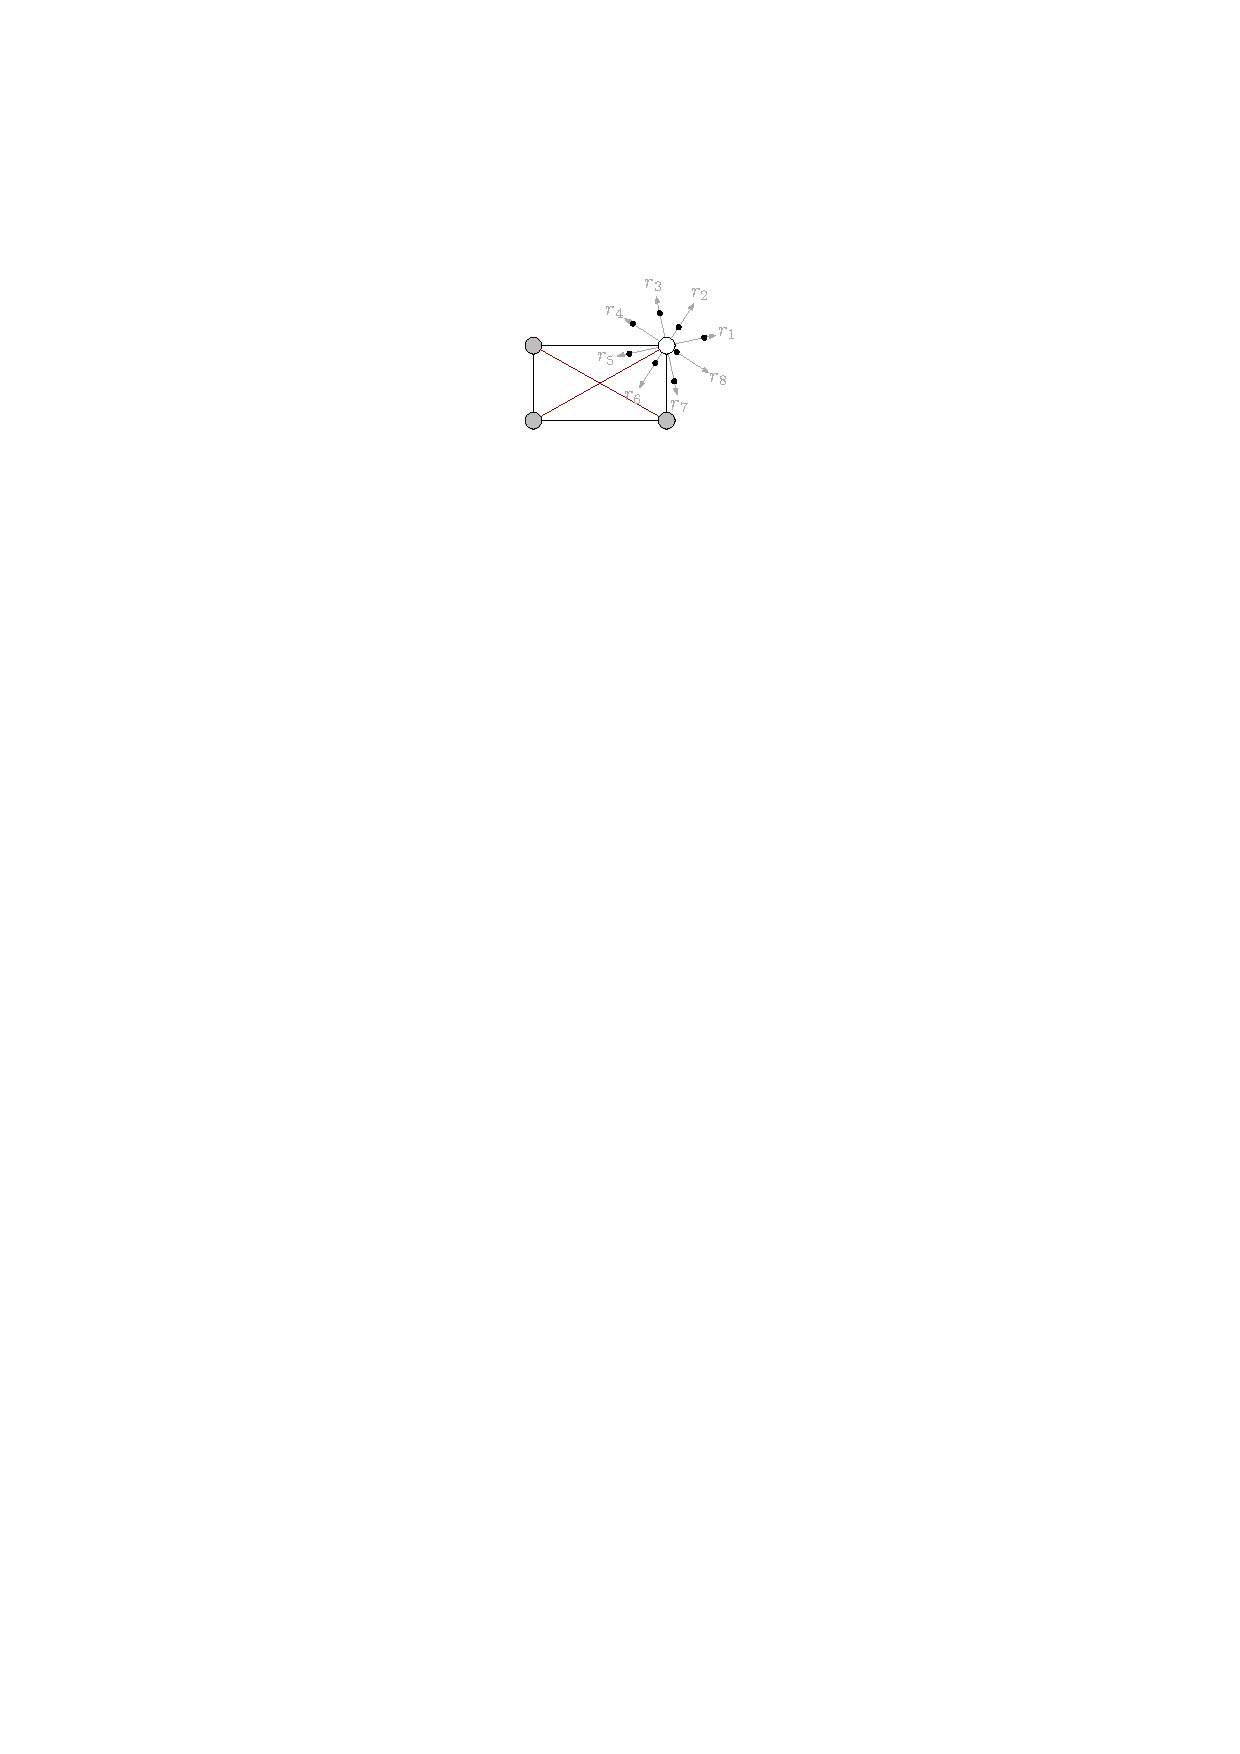
\includegraphics[page=1]{figures/algorithm}}
	\hfil
	\subfloat[\label{fig:algo-move} {}]{
	\includegraphics[page=2]{figures/algorithm}}
	\caption{%
	Illustration of an iteration step of our algorithm: 
	(a)~The chosen vertex is the white one; 
	the computed rays $r_0,\ldots,r_7$ have been rotated by $8^\circ$; 
	the black-colored points along these rays are points $\pi_0,\ldots,\pi_7$; 
	among them, $\pi_4$ yields the best solution.
	(b)~The resulting drawing after moving the vertex at position $\pi_2$.}
	\label{fig:algo}
\end{figure} 

If none of the points $\pi_j$, with $j=0,1,\ldots,\rho-1$ is feasible, then the new position of vertex $v_i$ in drawing $\Gamma_i$ is $p(v_i)$, that is, the same as in drawing $\Gamma_{i-1}$, since the crossing resolution of drawing $\Gamma_i$ must be at least as large as the one of $\Gamma_{i-1}$. On the other hand, if there is one or more feasible points (among $\pi_0,\pi_1,\ldots,\pi_{\rho-1}$), then one may consider two different approaches to determine the new position of vertex $v_i$ in drawing $\Gamma_i$. The most natural is to chose the feasible point that maximizes the crossing resolution of the obtained drawing. As an alternative, one may rely again on randomization and chose uniformly at random one of the feasible points as the new position of vertex $v_i$ in drawing $\Gamma_i$. In our implementation, we did not observe any significant difference in these two approaches (in terms of the crossing resolution of the obtained drawings), so we simply adopted the first one. In Section~\ref{ssec:termination}, we describe conditions under which we determine that our algorithm has converged.

\subsection{Avoiding local maxima.}
\label{ssec:maxima}

To avoid getting trapped to locally optimal solutions with the aforementioned procedure, we mainly investigated two different approaches. Both of them are parametrizable by two input parameters $\zeta$ and $\zeta'$. The first one mimics the human behaviour. What would one do to get away from a locally optimal solution? First, she would stop trying to move the endvertices of the edges defining the crossing resolution; she would start moving ``irrelevant'' vertices hoping that by changing the embedding of the graph or its crossing structure, a better solution would be easier to be computed again. Our algorithm is mimicking this idea by allowing the vertex-pool to also contain all the vertices of the graph, as follows: 

\begin{itemize}
%\item As long as the algorithm detects that within the last $\zeta$ iterations the crossing resolution of the graph has being improved, the vertex-pool contains only critical vertices. 
\item If during the last $\zeta$ iterations the crossing resolution has not been improved, then the vertex-pool becomes \emph{wider} containing all the vertices of the graph, and the algorithm is executed with this vertex-pool for $\zeta'$ iterations. 
\item After these $\zeta'$ iterations, the vertex-pool switches back to the critical vertices.
\end{itemize}
%
From our extensive practical analysis, we quickly realized that, while this approach turned out to be quite effective for medium-size graphs, for larger and denser graph, unfortunately, it was not so efficient. What we observed is that in larger graphs it was unlikely to change the embedding of the graph in a beneficial way for the algorithm to proceed, mainly because of the random choice of the vertices to be moved; in most iterations with the wider vertex-pool, the vertices chosen to be moved were not in the part of the drawing where the critical vertices resided.

The second approach that we investigated to avoid locally optimal solutions was based on the parameters $\rho$, $\delta_{min}$ and $\delta_{max}$ of the algorithm. Our idea was that if the algorithm gets trapped to a locally optimal solution, then a ``drastical'' or ``sharp'' move may help to get untrapped. We turned this idea into an algorithmic step as follows: 

\begin{itemize}
\item If during the last $\zeta$ iterations the crossing resolution has not been improved, we double the values of the parameters $\rho$, $\delta_{min}$ and $\delta_{max}$, and the algorithm is executed with these parameters for $\zeta'$ iterations.
\item After these $\zeta'$ iterations, the parameters $\rho$, $\delta_{min}$ and $\delta_{max}$ switch back to their initial (input) values.
\end{itemize}
%
Of course, this approach may lead to drawings with larger area, but this is somehow expected, as it turns out that drawings with high crossing resolution may require large drawing area; see, e.g.,~\cite{DBLP:journals/jgaa/AngeliniCDFBKS11,DBLP:journals/tcs/BrandenburgDEKL16}. 

\subsection{Conditions for termination.}
\label{ssec:termination}

The termination condition of our algorithm is simple and depends also on an input parameter $\tau$, such that $\tau \geq \zeta + \zeta'$. More precisely, if the crossing resolution during the last $\tau$ iterations has not been improved, then we assume that the algorithm has converged and we do not proceed any more.

\subsection{Complexity Related Issues.}
\label{ssec:complexity}

A critical factor that highly affects the efficiency of our algorithm is the computation of the crossing points among the edges (and the corresponding angles at these points, which determine the crossing resolution of the drawing). Given  a drawing, a naive approach to compute its crossing points requires $O(m^2)$ time, which can be slightly improved using a standard plane-sweep technique to $O(m \log m + c)$ time, where $m$ and $c$ are the number of edges and crossings of the drawing, respectively; refer, e.g., to~\cite{DBLP:books/lib/BergCKO08}. 

However, if the algorithm had to compute all crossing points and the corresponding angles at these points for each candidate position at each iteration step, then our algorithm would not be useful in practice. Instead, we adopted a different approach, which turned out to be quite efficient in practice. Recall that we denoted by $v_i$ the vertex chosen at the $i$-th iteration step, and by $\pi_0,\ldots,\pi_{\rho-1}$ the candidate points to move $v_i$. Let $e_0,\ldots,e_{d_i-1}$ be the edges incident to $v_i$, where $d_i=deg(v_i)$. Next, for each edge $e_k$ with $k=0,\ldots,d_i-1$  we compute the crossings and the corresponding crossing angles of $e_k$ with all other edges in drawing $\Gamma_{i-1}$. Let $\phi_i$ be the minimum crossing angle computed with this procedure; this is our reference angle. Also, for each candidate position $\pi_j$ with $j=0,\ldots,\rho-1$, and for each edge $e_k$ with $k=0,\ldots,d_i-1$, we compute the crossings and the corresponding crossing angles of $e_k$ with all other edges of the drawing, assuming that vertex $v_i$ is at position $\pi_j$. Let $\chi_j$ be the minimum crossing angle computed with this approach, when $v_i$ is at position $\pi_j$. Clearly, in our context, position $\pi_j$ is feasible only if $\chi_j \geq \phi_i$. Note that the complexity of this approach is $O(deg(v_i) \cdot m)$, which in worst-case is $O(nm)$. 

\subsection{Grid drawings: An interesting variant.}
\label{ssec:grid}

The algorithm, as it has been described so far, does not necessarily produce grid drawings, i.e., drawings in which the vertices are at integer coordinates. However, it can be easily adjusted to produce such drawings. Recall that, at the $i$-th iteration step, our algorithm chooses uniformly at random a vertex $v_i$ from the vertex-pool and determines a set of $\rho$ candidate points $\pi_0,\ldots,\pi_{\rho-1}$. If we round these points to their closest grid points, say $\overline{\pi}_0,\ldots,\overline{\pi}_{\rho-1}$, and use them as candidates for the next position of $v_i$, then the obtained drawing will be grid, assuming that the starting drawing is grid (the latter requirement is not difficult to be achieved, e.g., by slightly adjusting the positions of the vertices of a circular layout, whose underlying circle has large radius, to be at grid points). 

An alternative approach is to let our algorithm compute a (non-grid) drawing and then apply some technique to convert it to grid. Critical here is not to affect the crossing resolution too much during the conversion. Of course, if the crossing resolution of the obtained grid drawing is at least as large as the crossing resolution of the non-grid starting drawing, then we considered the computed grid drawing \emph{acceptable}. In our approach, we also accepted drawings whose crossing resolution is at least as large as the crossing resolution of the non-grid starting drawing minus an input parameter $\epsilon$, which we used as \emph{slack} for tolerating slightly worse solutions. For converting a non-grid drawing to grid, we repeated the following procedure, that is also based on randomization, until we compute an acceptable grid drawing: For each vertex of the non-grid starting drawing, chose uniformly at random one of the grid points from the so-called \emph{neighbourhood} of the vertex, and move the vertex to this point (assuming of course that there is no other vertex at this point), where the neighbourhood of a vertex was initially set to its four closest grid points. If after a number of iterations an acceptable grid drawing without vertex-vertex overlaps could not be reported, then we augmented the neighbourhood of all vertices to contain more grid points, in particular, the grid points that are in horizontal and vertical distance~$1$ from the grid points of the current neighborhood. 


\section{Experimental Evaluation}
\label{sec:experiments}

\begin{itemize}
\item Experimental setup.
\item Benchmarks + degree-3.
\item Aesthetics:

\begin{itemize}
\item Number of crossings (\# of crossings).
\item Average size of crossing angles (angle size).
\item Average of edge lengths (edge length).
\item Angular resolution (angular res.).
\end{itemize}

\item Results.
\item Discussion.
\end{itemize}

\section{Conclusions}
\label{sec:conclusions}

\bibliographystyle{abbrvurl}
\bibliography{references}

\end{document}
